\chapter{Evaluation}
\label{sec:eval}

In this section, we evaluate our design choices in building Consistent
and Durable Data Structures.  First, we measure the overhead
associated with techniques used to achieve durability on existing
processors.  We then compare the CDDS B-tree to Berkeley DB and
against log-based schemes.  After briefly discussing CDDS
implementation and integration complexity, we present results from a
multi-node distributed experiment where we use the Yahoo Cloud Serving
Benchmark (YCSB)~\citep{Cooper10}.
% to compare Tembo to Cassandra~\citep{Lakshman10}.

\section{Evaluation Setup}

% HP Proliant DL360 G6

As NVBM is not commercially available yet, we used DRAM-based servers.
While others~\citep{Condit09} have shown that DRAM-based results are a good
predictor of NVBM performance, as a part of our ongoing work, we aim
to run micro-architectural simulations to confirm this within the
context of our work.  Our testbed consisted of 15 servers with two
Intel Xeon Quad-Core 2.67~GHz (X5550) processors and 48~GB RAM each.
The machines were connected via a full-bisection Gigabit Ethernet 
network.  Each processor has 128~KB L1, 256~KB L2, and 8~MB L3 caches.
While each server contained 8 300~GB 10K SAS drives, unless specified,
all experiments were run directly on RAM or on a ramdisk.  We
used the Ubuntu~10.04 Linux distribution and the 2.6.32-24 64-bit
kernel.

%  1333~MHz RAM. If you look at the processor specs, this becomes
%  clear.


\section{Flush Performance}
\label{sec:flush_perf}

\begin{figure}[t]
\begin{minipage}[b]{0.49\linewidth}
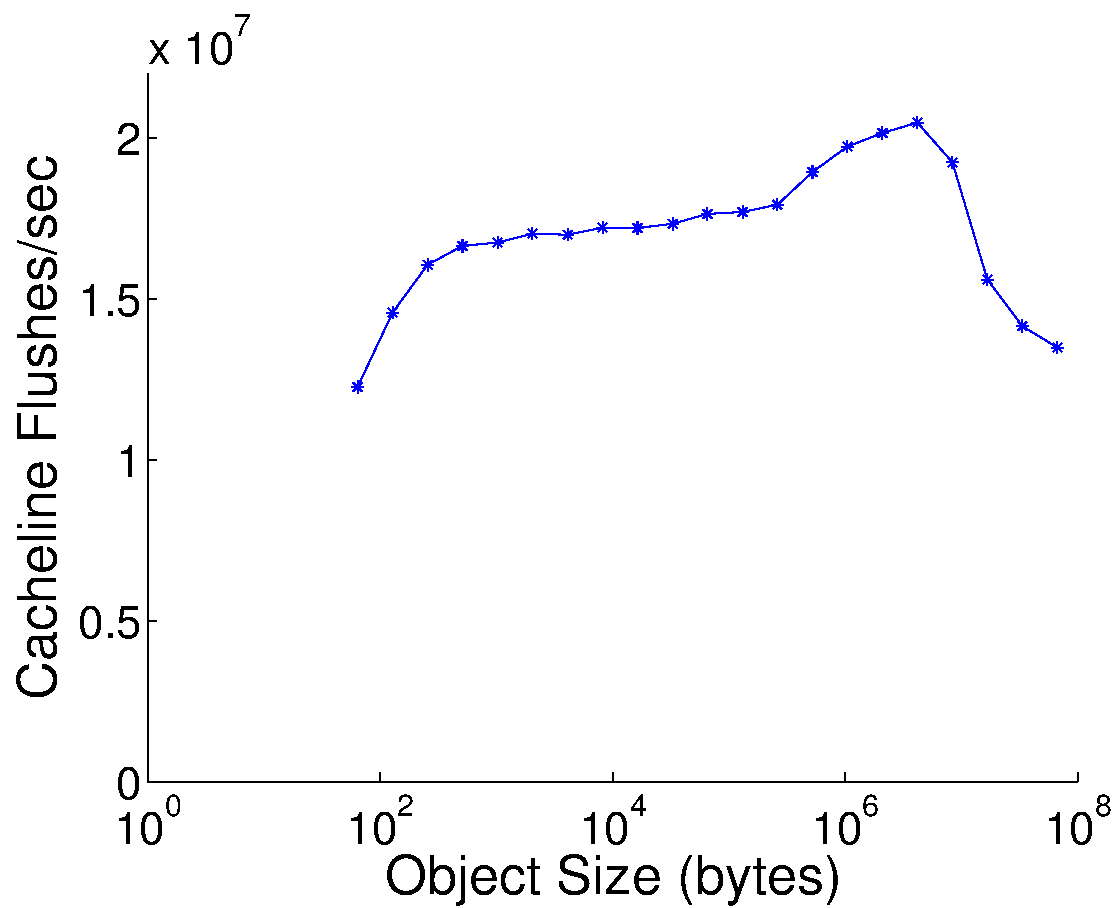
\includegraphics[width=\columnwidth]{figs/flushes_per_sec}
%\vspace{-0.3in}
\caption{Flushes/second}
\label{fig:flushes_per_sec}
\end{minipage}
%\hspace{0.1cm}
\begin{minipage}[b]{0.49\linewidth}
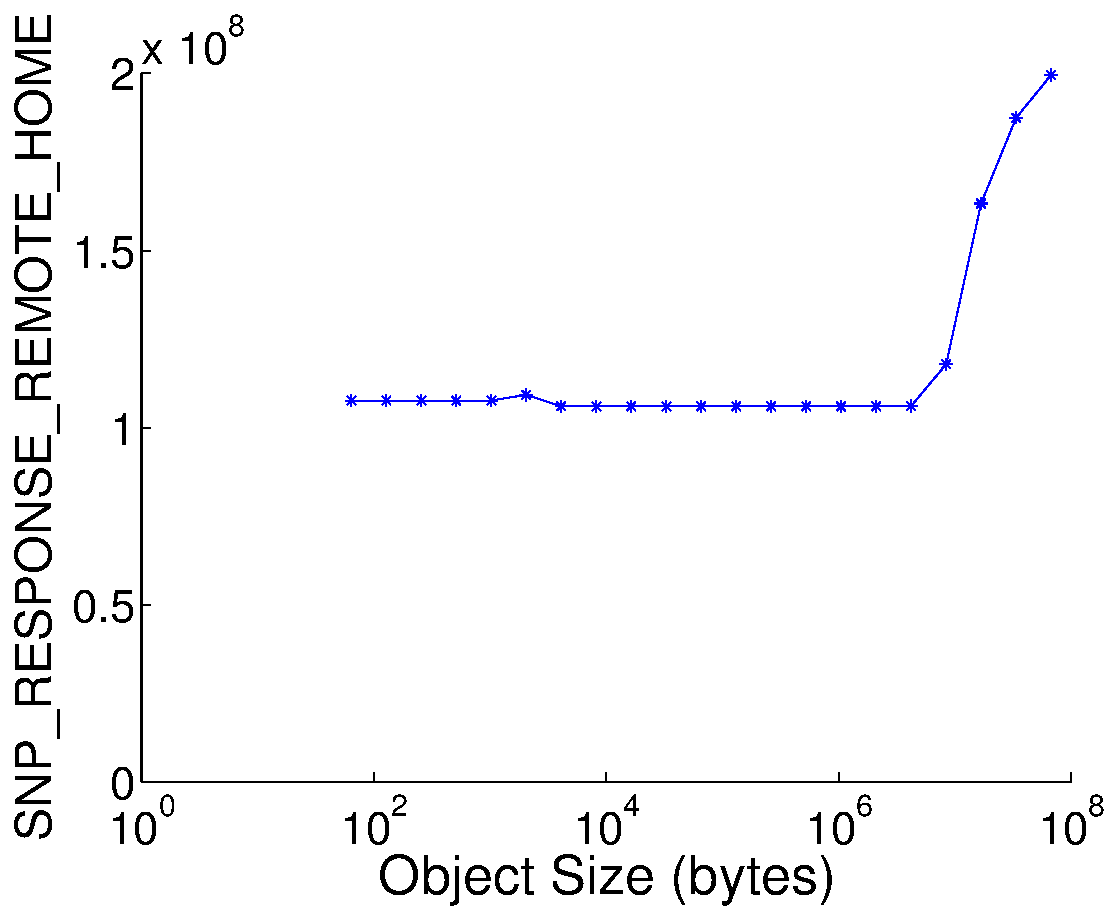
\includegraphics[width=\columnwidth]{figs/snoop_response}
%\vspace{-0.3in}
\caption{Cache Snooping}
\label{fig:ext_snoop}
\end{minipage}
%\vspace{-0.15in}
\end{figure}

To accurately capture the performance of the \texttt{flush} operation
defined in Chapter~\ref{sec:flush}, we used the ``MultCallFlushLRU''
methodology~\citep{Whaley08}.  The experiment allocates 64~MB of
memory and subdivides it into equally-sized cache-aligned objects.
Object sizes ranged from 64~bytes to 64~MB\@.  We write to every
cache line in an object, \texttt{flush} the entire object, and then
repeat the process with the next object.  For improved timing
accuracy, we stride over the memory region multiple times.

Remembering that each \texttt{flush} is a number of \texttt{clflush}es
bracketed by \texttt{mfence}s on both sides,
Figure~\ref{fig:flushes_per_sec} shows the number of
\texttt{clflush}es executed per second.  Flushing small objects sees
the worst performance ($\sim$12M cacheline flushes/sec for 64~byte
objects).  For larger objects (256~bytes--8~MB), the performance
ranges from $\sim$16M--20M cacheline flushes/sec.

\begin{sloppypar}
We also observed an unexpected drop in performance for large objects
($>$8~MB).  Our analysis showed that this was due to the cache
coherency protocol.  Large objects are likely to be evicted from the
L3 cache before they are explicitly flushed. A subsequent
\texttt{clflush} would miss in the local cache and cause a
high-latency ``snoop'' request that checks the second off-socket
processor for the given cache line.  As measured by the
UNC\_SNP\_RESP\_TO\_REMOTE\_HOME.I\_STATE performance counter, seen in
Figure~\ref{fig:ext_snoop}, the second socket shows a corresponding
spike in requests for cache lines that it does not contain.  To verify
this, we physically removed a processor and observed that the anomaly
disappeared\footnote{We did not have physical access to the
  experimental testbed and ran the processor removal experiment on a different
  dual-socket Intel Xeon (X5570) machine.}.  Further, as we could not
replicate this slowdown on AMD platforms, we believe that
cache-coherency protocol modifications can address this anomaly.
\end{sloppypar}

%These results show that \texttt{flush}'s performance is acceptable for
%most workloads because, unlike the artificial tight loop in this
%experiment, \texttt{flush}es are generally batched and only invoked
%when data needs to be made durable.

Overall, the results show that we can \texttt{flush} 0.72--1.19~GB/s
on current processors.  For applications without networking,
Chapter~\ref{sec:api_microbench} shows that future hardware support
can help but applications using \texttt{flush} can still outperform
applications that use file system \texttt{sync} calls.  Distributed
applications are more likely to encounter network bottlenecks before
\texttt{flush} becomes an overhead.
%  Alternatively, a smarter implementation could interleave the
%  \texttt{clflush} and \texttt{fence} for large objects.

\section{API Microbenchmarks}
\label{sec:api_microbench}

\begin{figure}[t]
\begin{minipage}[b]{0.49\textwidth}
\centerline{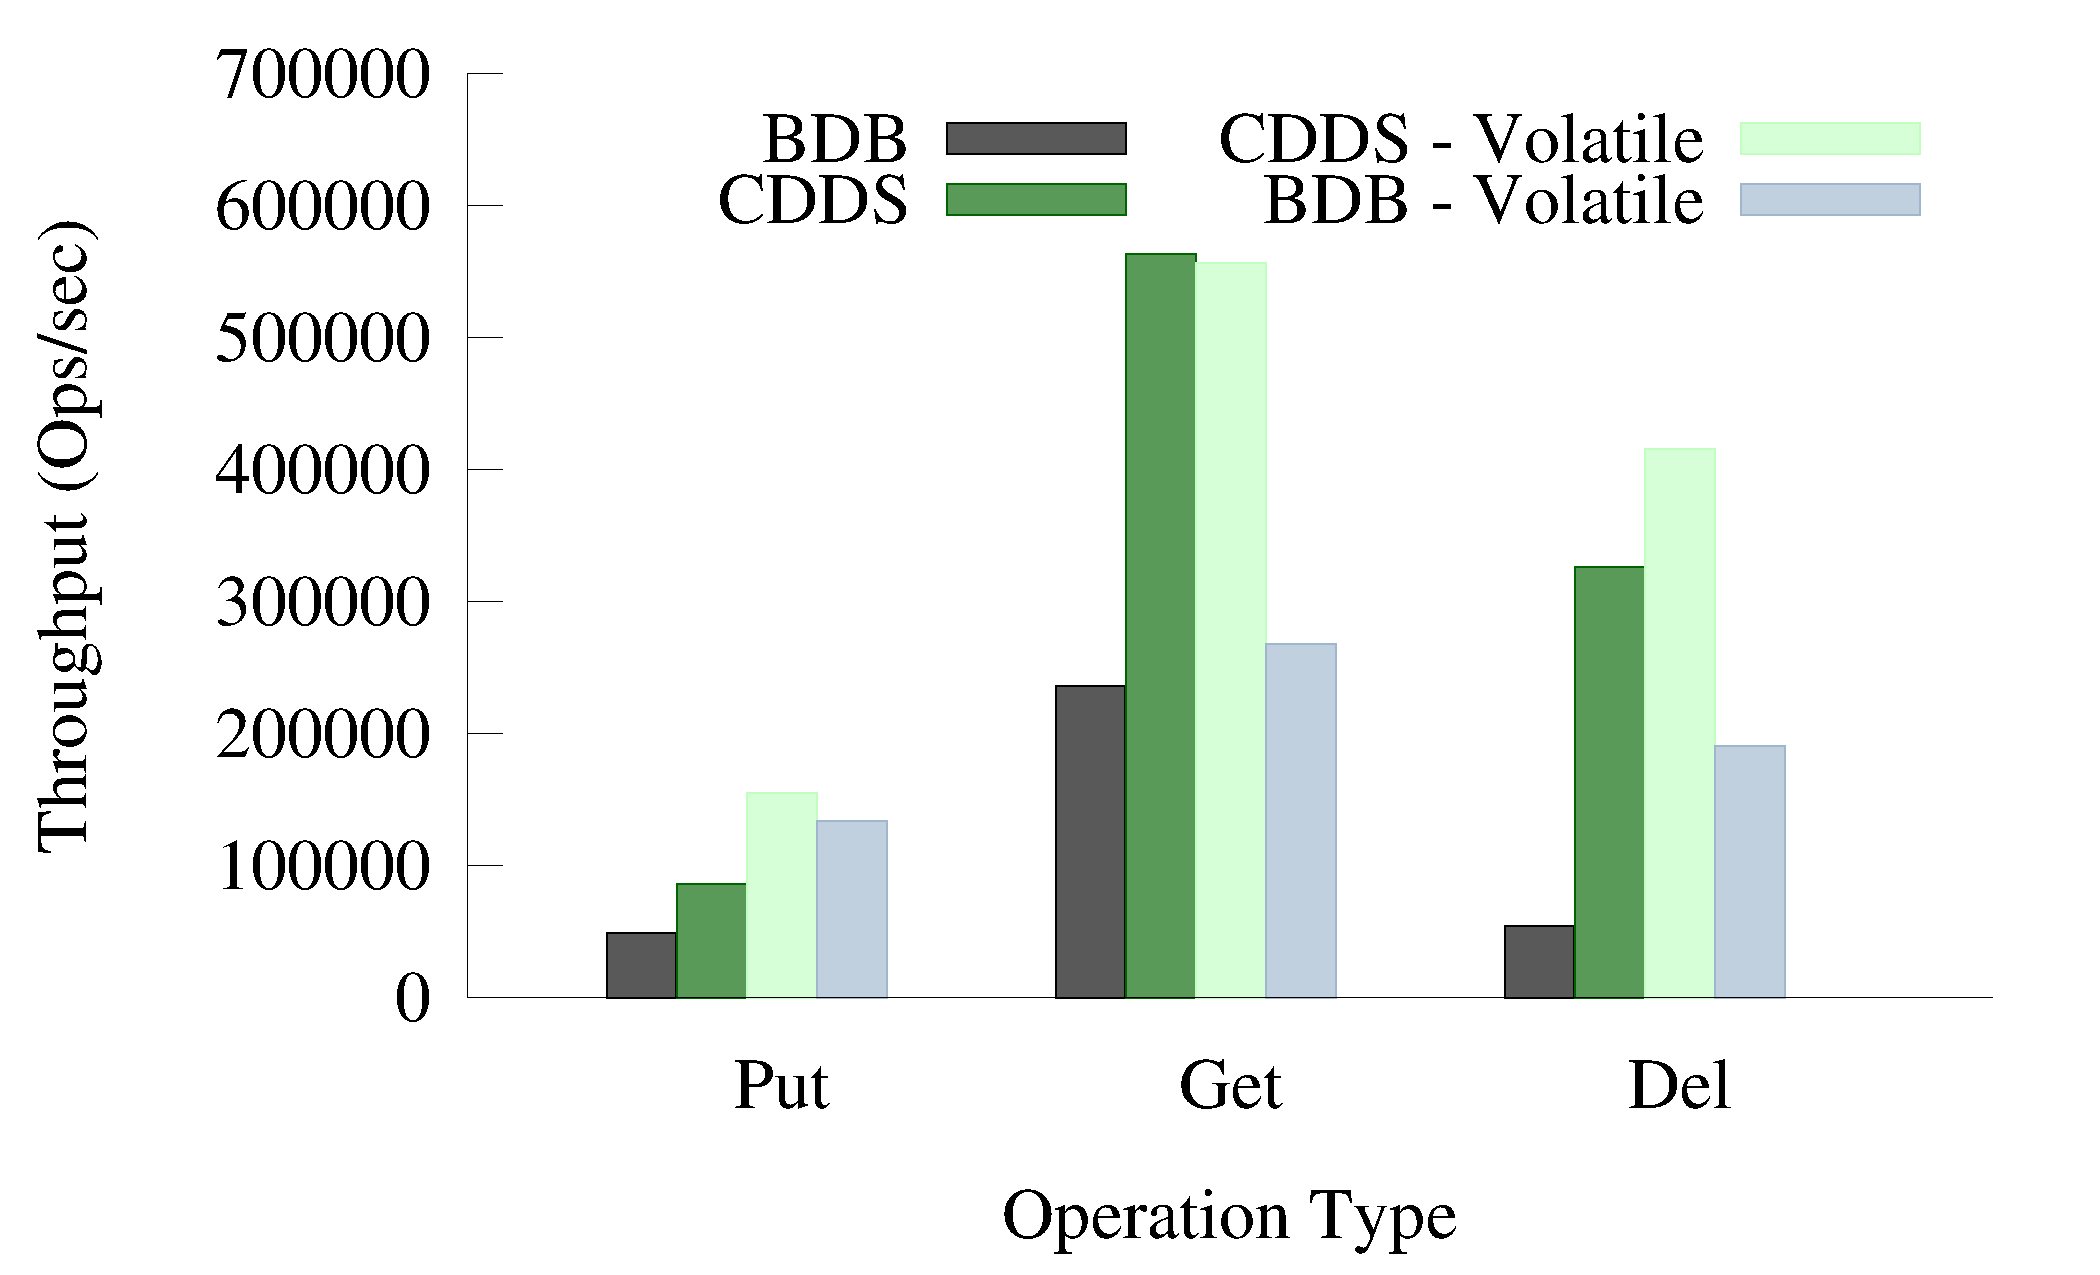
\includegraphics[width=\columnwidth]{figs/bdb-bench}}
\begin{captiontext}
\centerline{Mean of 5 trials. Max.\ standard deviation:
  2.2\% of the mean.}
\end{captiontext}
\caption{Berkeley DB Comparison}
\label{fig:bdb}
\end{minipage}
\begin{minipage}[b]{0.49\textwidth}
\centerline{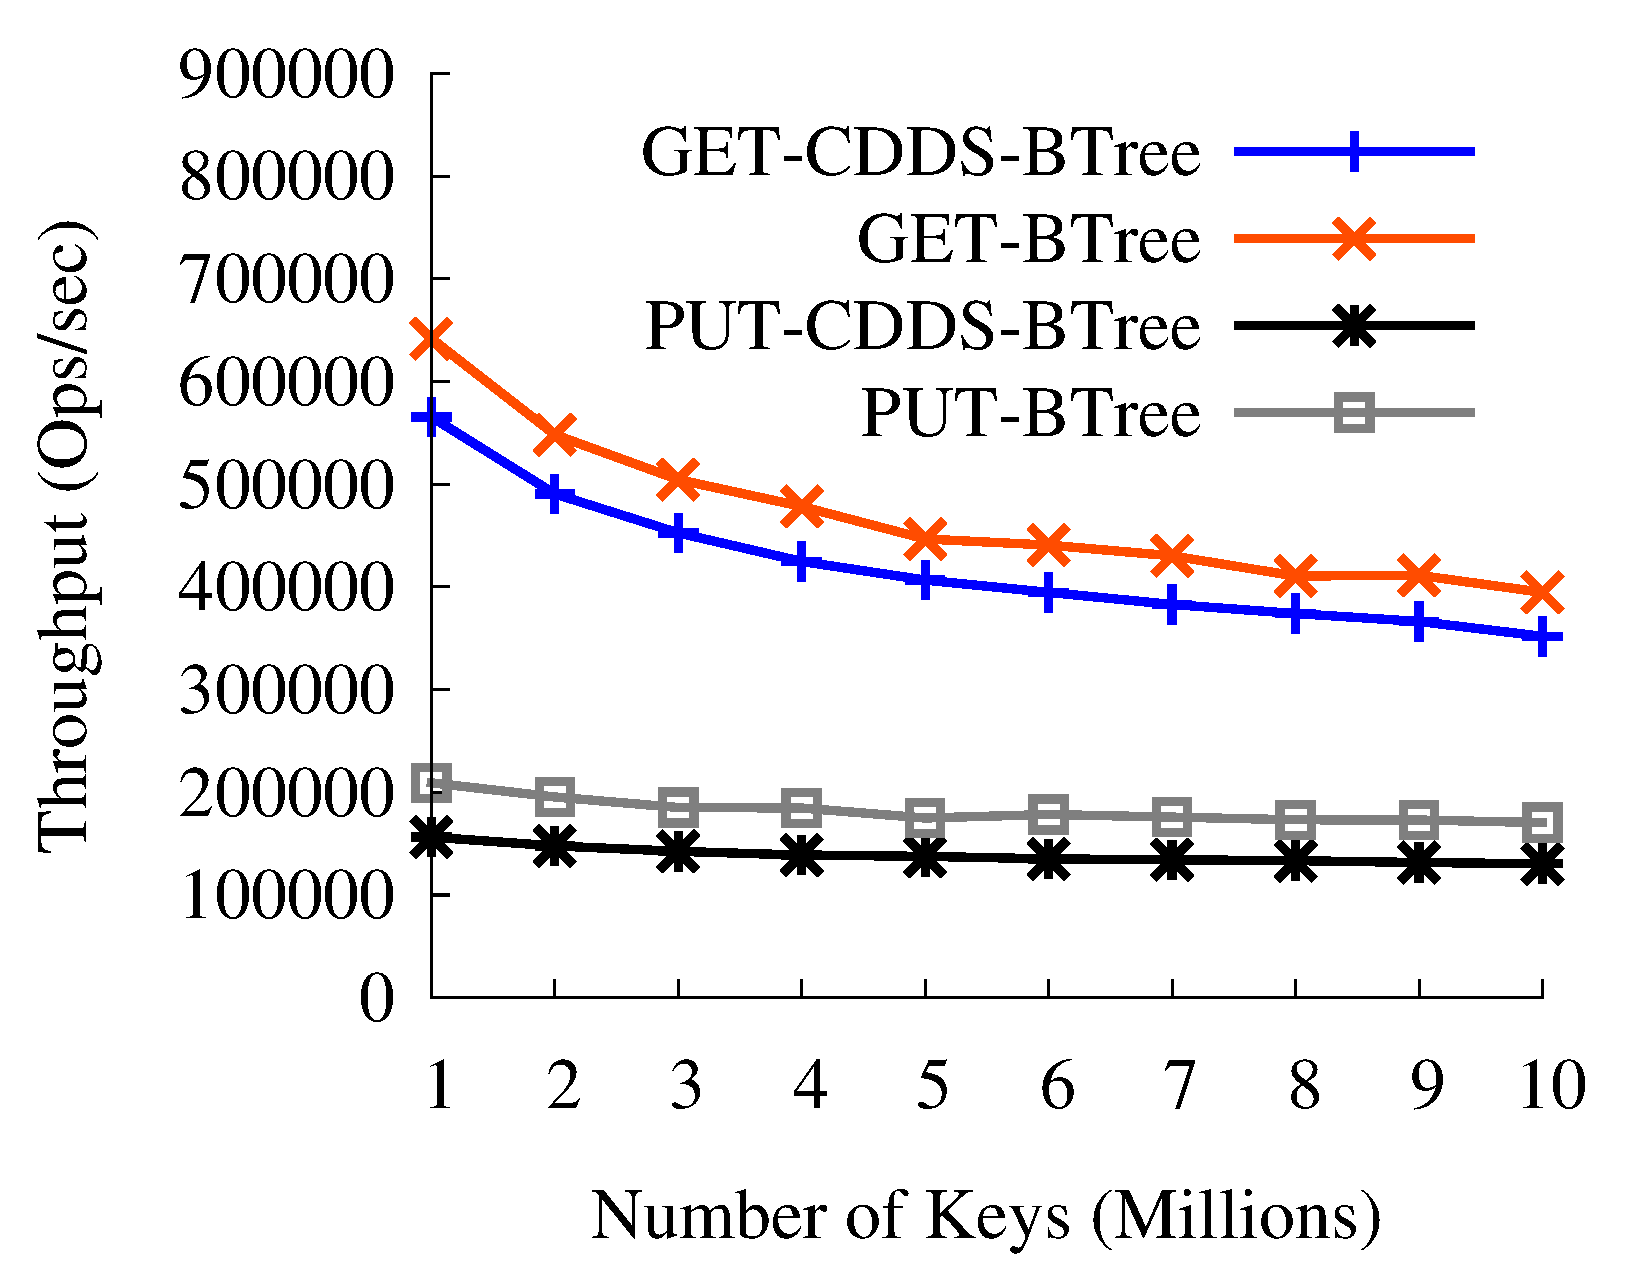
\includegraphics[width=0.85\columnwidth]{figs/versioning}}
%\begin{captiontext}
%\centerline{Mean of 5 trials. Max.\ standard deviation:
% 2.2\% of the mean.}
%\end{captiontext}
\caption{Versioning Overhead}
\label{fig:overhead}
\end{minipage}
\end{figure}

This section compares the CDDS B-Tree performance for puts, gets, and
deletes to Berkeley DB's (BDB) B-Tree implementation~\citep{Olson99}.
For this experiment, we insert, fetch, and then delete 1~million
key-value tuples into each system.  After each operation, we flush
the CPU cache to eliminate any variance due to cache contents.
Keys and values are 25 and 2048~bytes large.  The single-threaded
benchmark driver runs in the same address space as BDB and CDDS\@.
BDB's cache size was set to 8~GB and could hold the entire data
set in memory. Further, we configure BDB to maintain its log files
on an in-memory partition.

We run both CDDS and BDB (v4.8) in durable and volatile modes.  For
BDB volatile mode, we turn transactions and logging off.  For CDDS
volatile mode, we turn \texttt{flush}ing off.  Both systems in
volatile mode can lose or corrupt data and would not be used where
durability is required.  We only present the volatile results to
highlight predicted performance if hardware support was available and
to discuss CDDS design tradeoffs.

The results, displayed in Figure~\ref{fig:bdb}, show that, for
memory-backed BDB in durable mode, the CDDS B-Tree improves throughout
by 74\%, 138\%, and 503\% for puts, gets, and deletes respectively.
These gains come from not using a log (extra writes) or the file
system interface (system call overhead).  CDDS delete improvement is
larger than puts and gets because we do not delete data immediately
but simply mark it as dead and use GC to free unreferenced memory.  In
results not presented here, reducing the value size, and therefore the
log size, improves BDB performance but CDDS always performs better.

% XXX - Can we verify the 7\% improvement reason?

If zero-overhead epoch-based hardware support~\citep{Condit09} was
available, the CDDS volatile numbers show that performance of puts
and deletes would increase by 80\% and 27\% as \texttt{flush}es
would never be on the critical path. We do not observe any significant
change for gets as the only difference between the volatile and durable
CDDS is that the \texttt{flush} operations are converted into a noop.
%  We are still examining the reasons for the
% 6\% performance improvement in get operations but believe it to be a
% result of \texttt{flush} behavior.  As the puts immediately precede
% the gets, \texttt{flush}es in the durable case invalidate cache lines
% and they need to be brought back into cache for the next access.
% However, with the volatile CDDS, no \texttt{flush}es are used and the
% cache is warm for the get portion of the experiment.

% We see a large difference for delete performance because, as explained
% in Chapter~\ref{sec:btree_delete}, the durable CDDS B-Tree can create
% new nodes and invokes additional \texttt{flush}es.

We also notice that while volatile BDB throughput is lower than
durable CDDS for gets and dels by 52\% and 41\%, it is higher by 56\%
for puts.  Puts are slower for the CDDS B-Tree because of the work
required to maintain key ordering (described in
Chapter~\ref{sec:btree_lookup}), GC overhead, and a slightly higher
height due to nodes with a mixture of live and dead entries.  Volatile
BDB throughput is also higher than durable BDB but lower than volatile
CDDS for all operations.

To measure versioning overhead, we compared the volatile CDDS
B-Tree to a normal B-Tree~\citep{Bingman08}.  We performed the same
experiment described above and varied the input from one to
ten million keys. From the results, shown in Figure~\ref{fig:overhead},
we can see that the performance of the CDDS-BTree remains consistent
as we increase the number of keys. Also, we can see that volatile
CDDS's performance was lower than the in-memory B-Tree by 21\%-25\%
for puts and by 9\%-12\% for gets. This difference is similar to other
performance-optimized versioned B-trees~\citep{Soules03}.

% Put performance - BDB has no GC
% Get performance - BDB better because of smaller height tree

% 1. BDB Put is sensitive to value size. Decreasing value size reduces
% the performance difference.

% 2. CDDS (both) and B-tree (vanilla + not presented here) VERY
% sensitive to comparator.

% 3. Key size matters a lot for the delete. Reason is unverified but
% could be that CDDS does not erase value memory. GC does that.


\section{Implementation Effort}
\label{sec:impl_effort}



The CDDS B-Tree started with the STX C++ B-Tree~\citep{Bingman08}
implementation but, as measured by \texttt{sloccount} and shown in
Table~\ref{tab:integration}, the addition of versioning and NVBM
durability replaced 90\% of the code.  While the API remained the
same, the internal implementation differs substantially.  The
integration with Redis to create Tembo was simpler and only changed
1.7\% of code and took less than a day to integrate.  Since the CDDS
B-Tree implements an interface similar to an STL Sorted Container, we
believe that integration with other systems should also be simple.
Overall, our experiences show that while the initial implementation
complexity is moderately high, this only needs to be done once for a
given data structure.  The subsequent integration into legacy
or new systems is straightforward.


\section{Tembo Versioning vs.\ Redis Logging}
\label{sec:versioning_logging}

\begin{table}[t]
\begin{minipage}[b]{0.49\textwidth}
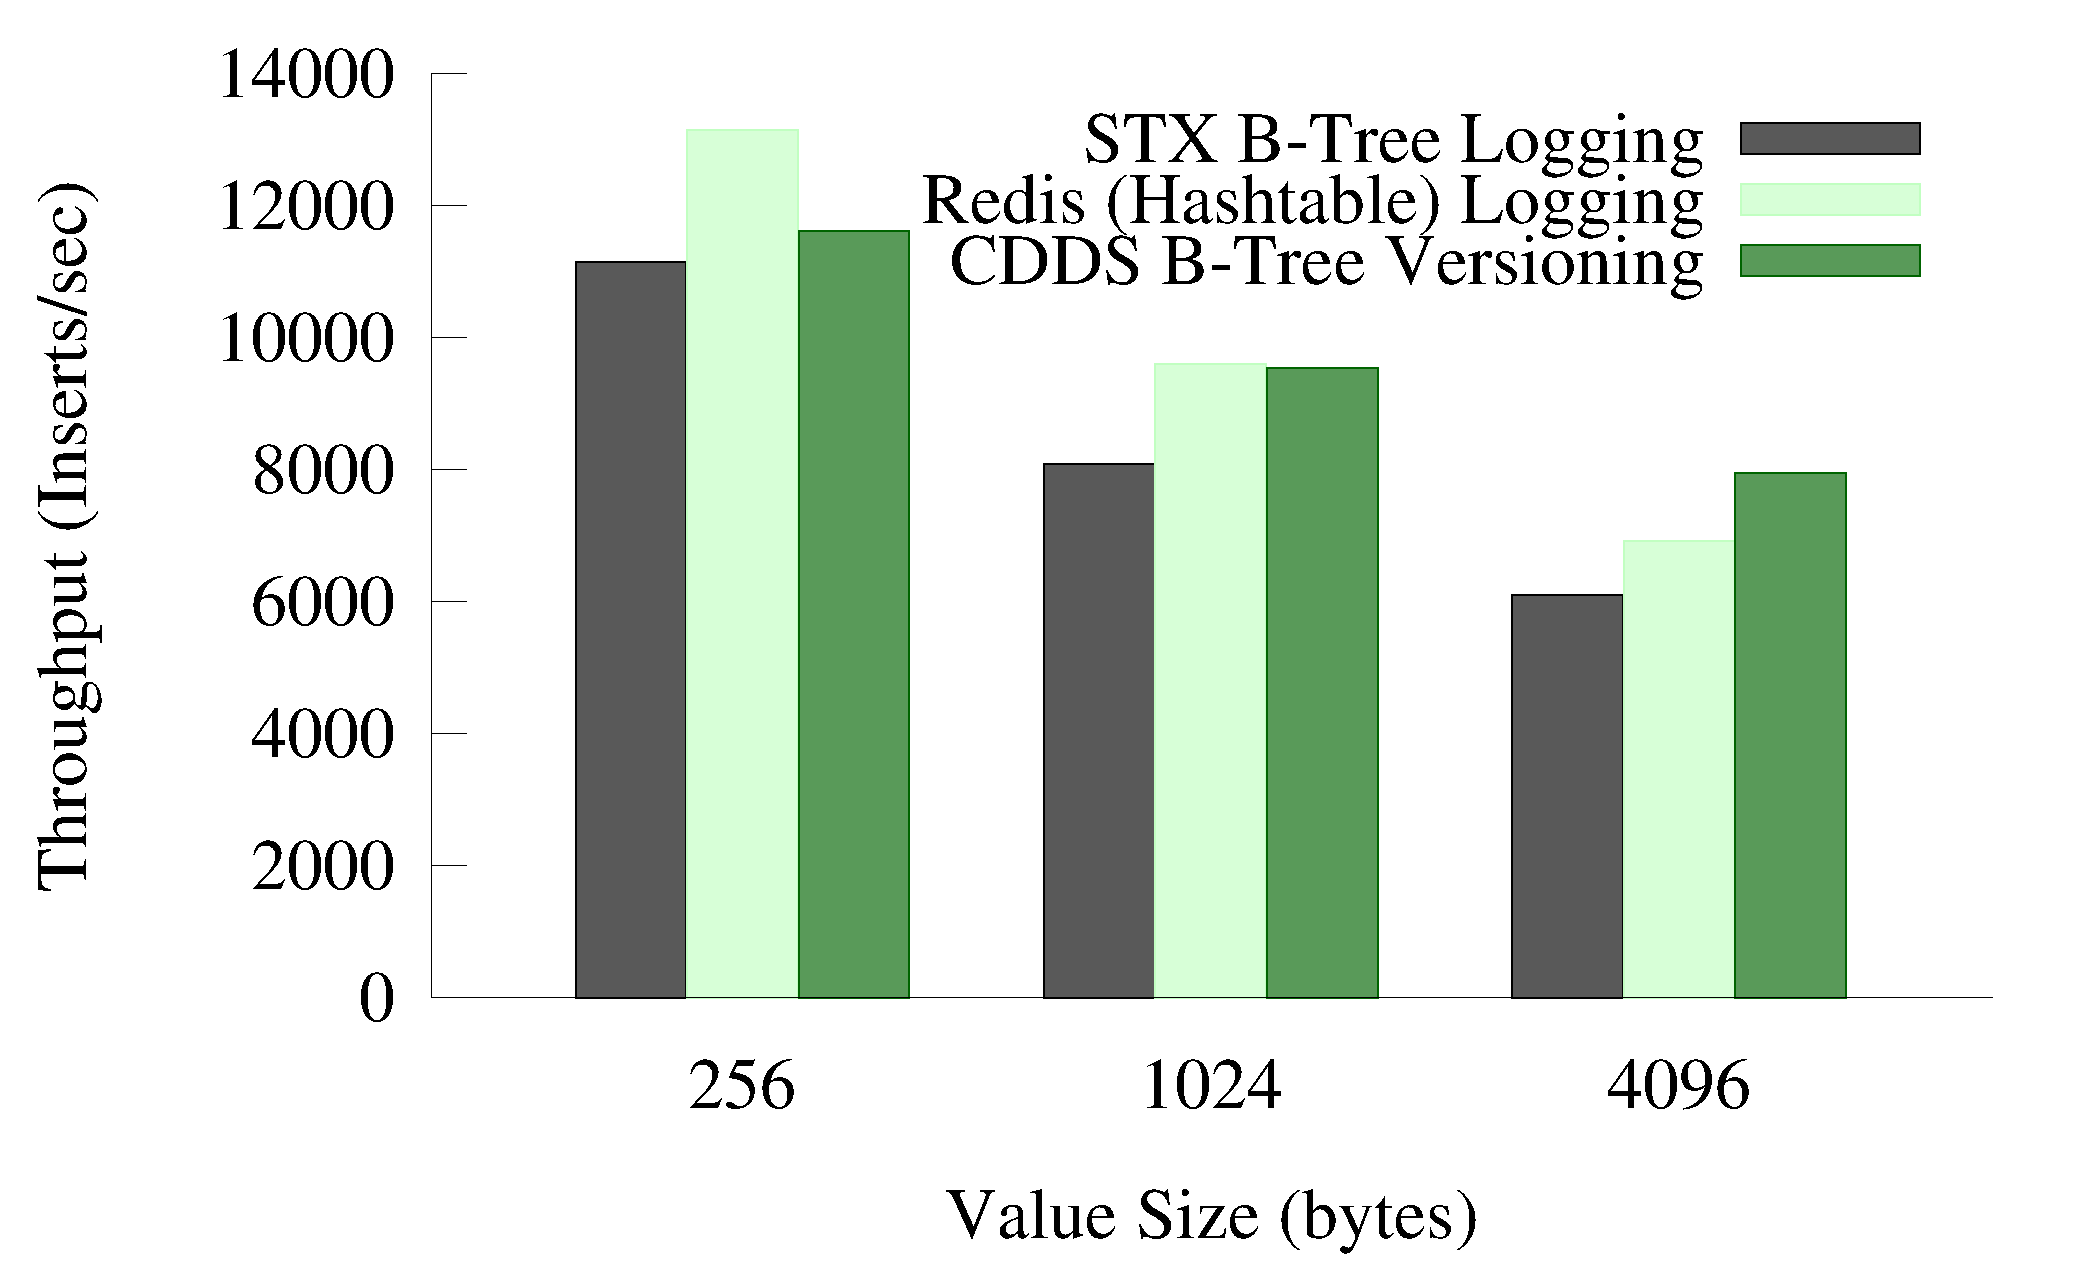
\includegraphics[width=\columnwidth]{figs/durability}
\begin{captiontext}
\centerline{Mean of 5 trials. Max.\ standard deviation: 6.7\% of the mean.}
\end{captiontext}
\captionof{figure}{Versioning vs.\ Logging}
\label{fig:durability}
\end{minipage}
\begin{minipage}[b]{0.49\textwidth}
\centerline{
\begin{tabular}{c|c}
                      & Lines of Code \\ \hline \hline
Original STX B-Tree   & 2,110         \\                 % Only include dir
CDDS Modifications    & 1,902         \\ \hline \hline
Redis (v2.0.0-rc4)               & 18,539        \\
Tembo Modifications   & 321              
\end{tabular}
}
\caption{Lines of Code Modified}
\label{tab:integration}
\end{minipage}
\end{table}




Apart from the B-Tree specific logging performed by BDB in
Chapter~\ref{sec:api_microbench}, we also wanted to compare CDDS
versioning when integrated into Tembo to the write-ahead log used by
Redis in fully-durable mode.  Redis uses a hashtable and, as it is
hard to compare hashtables and tree-based data structures, we also
replaced the hashtable with the STX B-Tree. In this single-node
experiment, we used 6~Tembo or Redis data stores and 2
clients\footnote{Being event-driven, both Redis and Tembo are
  single-threaded. Therefore one data store (or client) is run per core
  in this experiment.}.  The write-ahead log for the Redis server was
stored on an in-memory partition mounted as \texttt{tmpfs} and did not
use the hard disk. Each client performed 1M inserts over the
loopback interface.

The results, presented in Figure~\ref{fig:durability}, show that as
the value size is increased, Tembo performs up to 30\% better than
Redis integrated with the STX B-Tree.  While Redis updates the
in-memory data copy and also writes to the append-only log, Tembo only
updates a single copy.  While hashtable-based Redis is faster than
Tembo for 256~byte values because of faster lookups, even
with the disadvantage of a tree-based structure, Tembo's performance
is almost equivalent for 1~KB values and is 15\% faster for 4~KB
values.

The improvements for the experiments in this section are lower than those in
Chapter~\ref{sec:api_microbench} because of network latency overhead.  The
\texttt{fsync} implementation in \texttt{tmpfs} also does not explicitly flush
modified cache lines to memory and is therefore biased against Tembo.  We are
working on modifications to the file system that will enable a fairer
comparison.  Finally, some of the overhead is due to maintaining ordering
properties in the CDDS-based B-Tree to support range scans - a feature not used
in the current implementation of Tembo.

%one should note that Tembo does not utilize all
%features of the CDDS B-Tree, including range scans and iterator
%support.  Tembo's evaluation is therefore biased against CDDSs because
%it pays the runtime overhead for these features but does not use them.

\begin{figure}[t]
\begin{minipage}[b]{0.49\textwidth}
\centerline{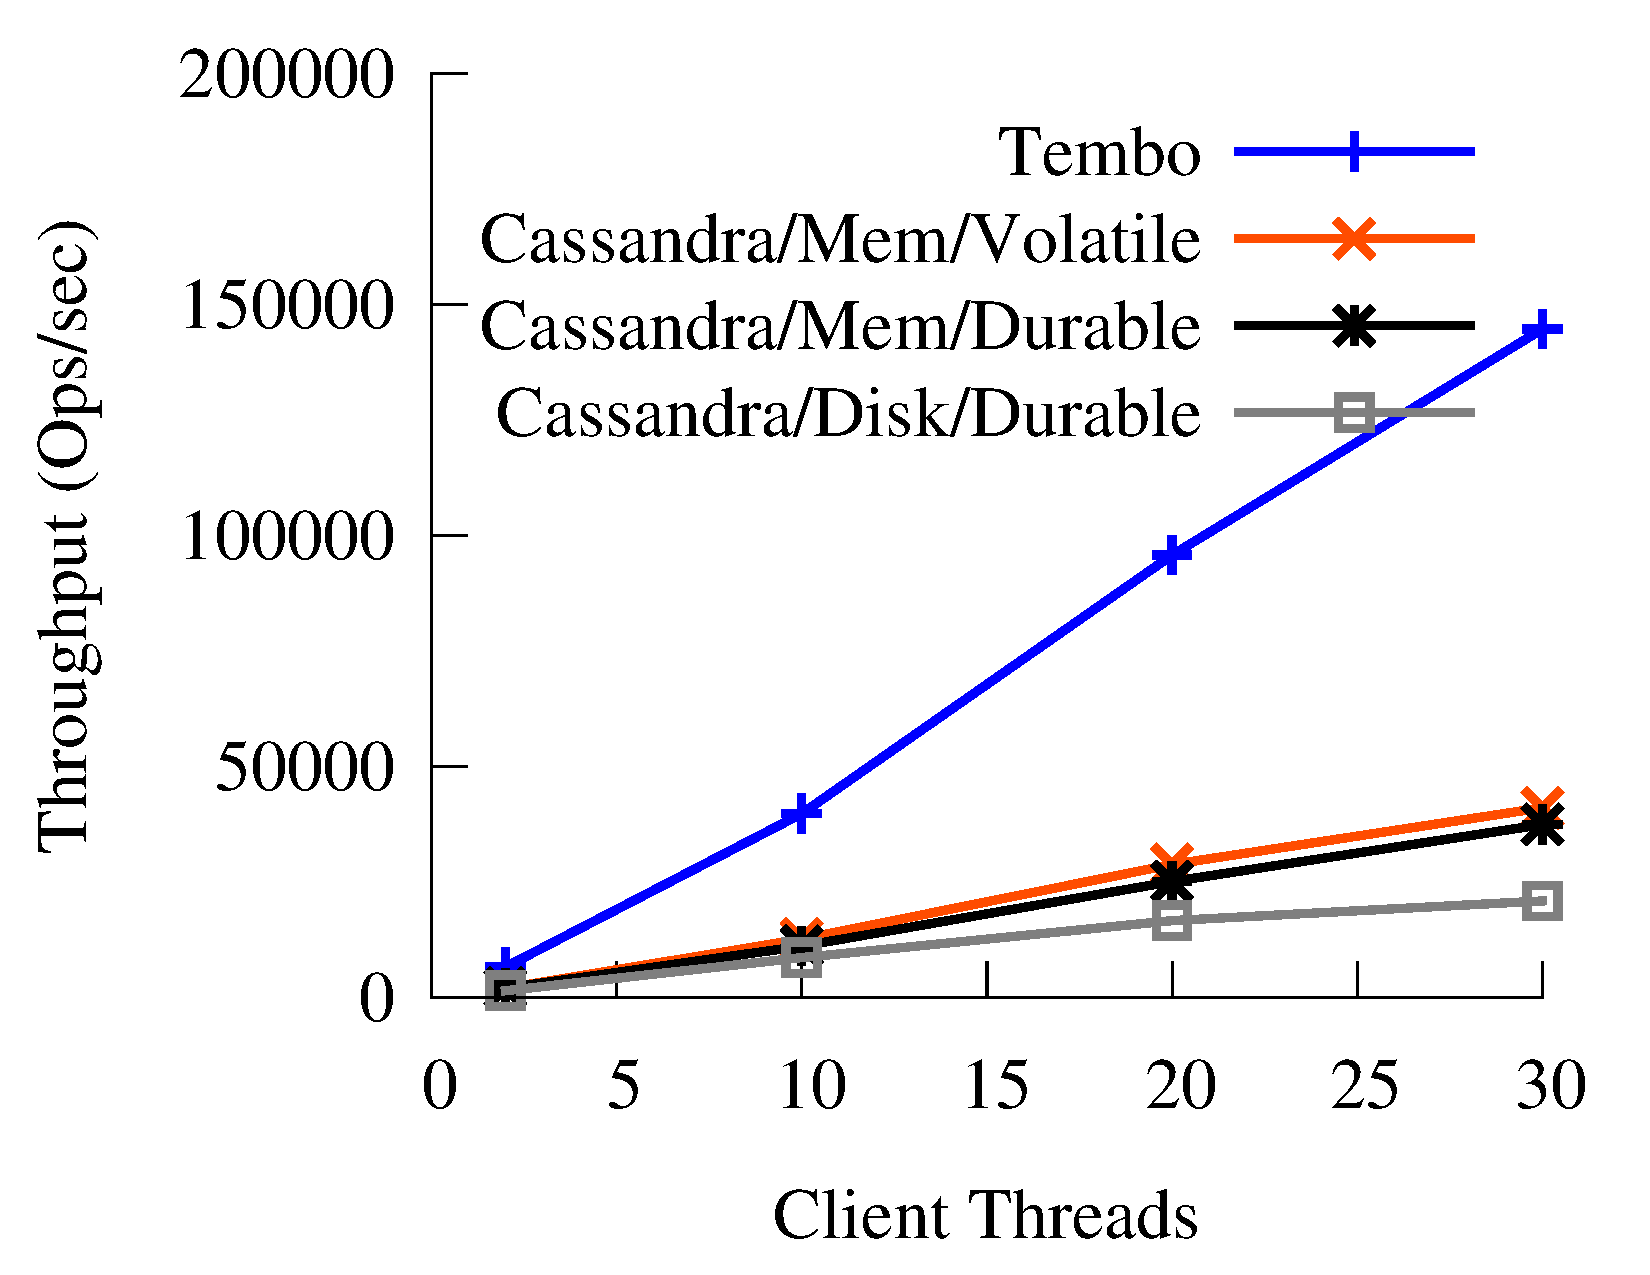
\includegraphics[width=0.85\columnwidth]{figs/ycsb-a}}
\begin{captiontext}
 \centerline{Mean of 5 trials. Max.\ standard deviation: 7.8\% of the
   mean.}
\end{captiontext}
\caption[Yahoo Cloud Serving Benchmark: SessionStore]{YCSB: SessionStore}
\label{fig:ycsb_session_store}
\end{minipage}
\begin{minipage}[b]{0.49\textwidth}
\centerline{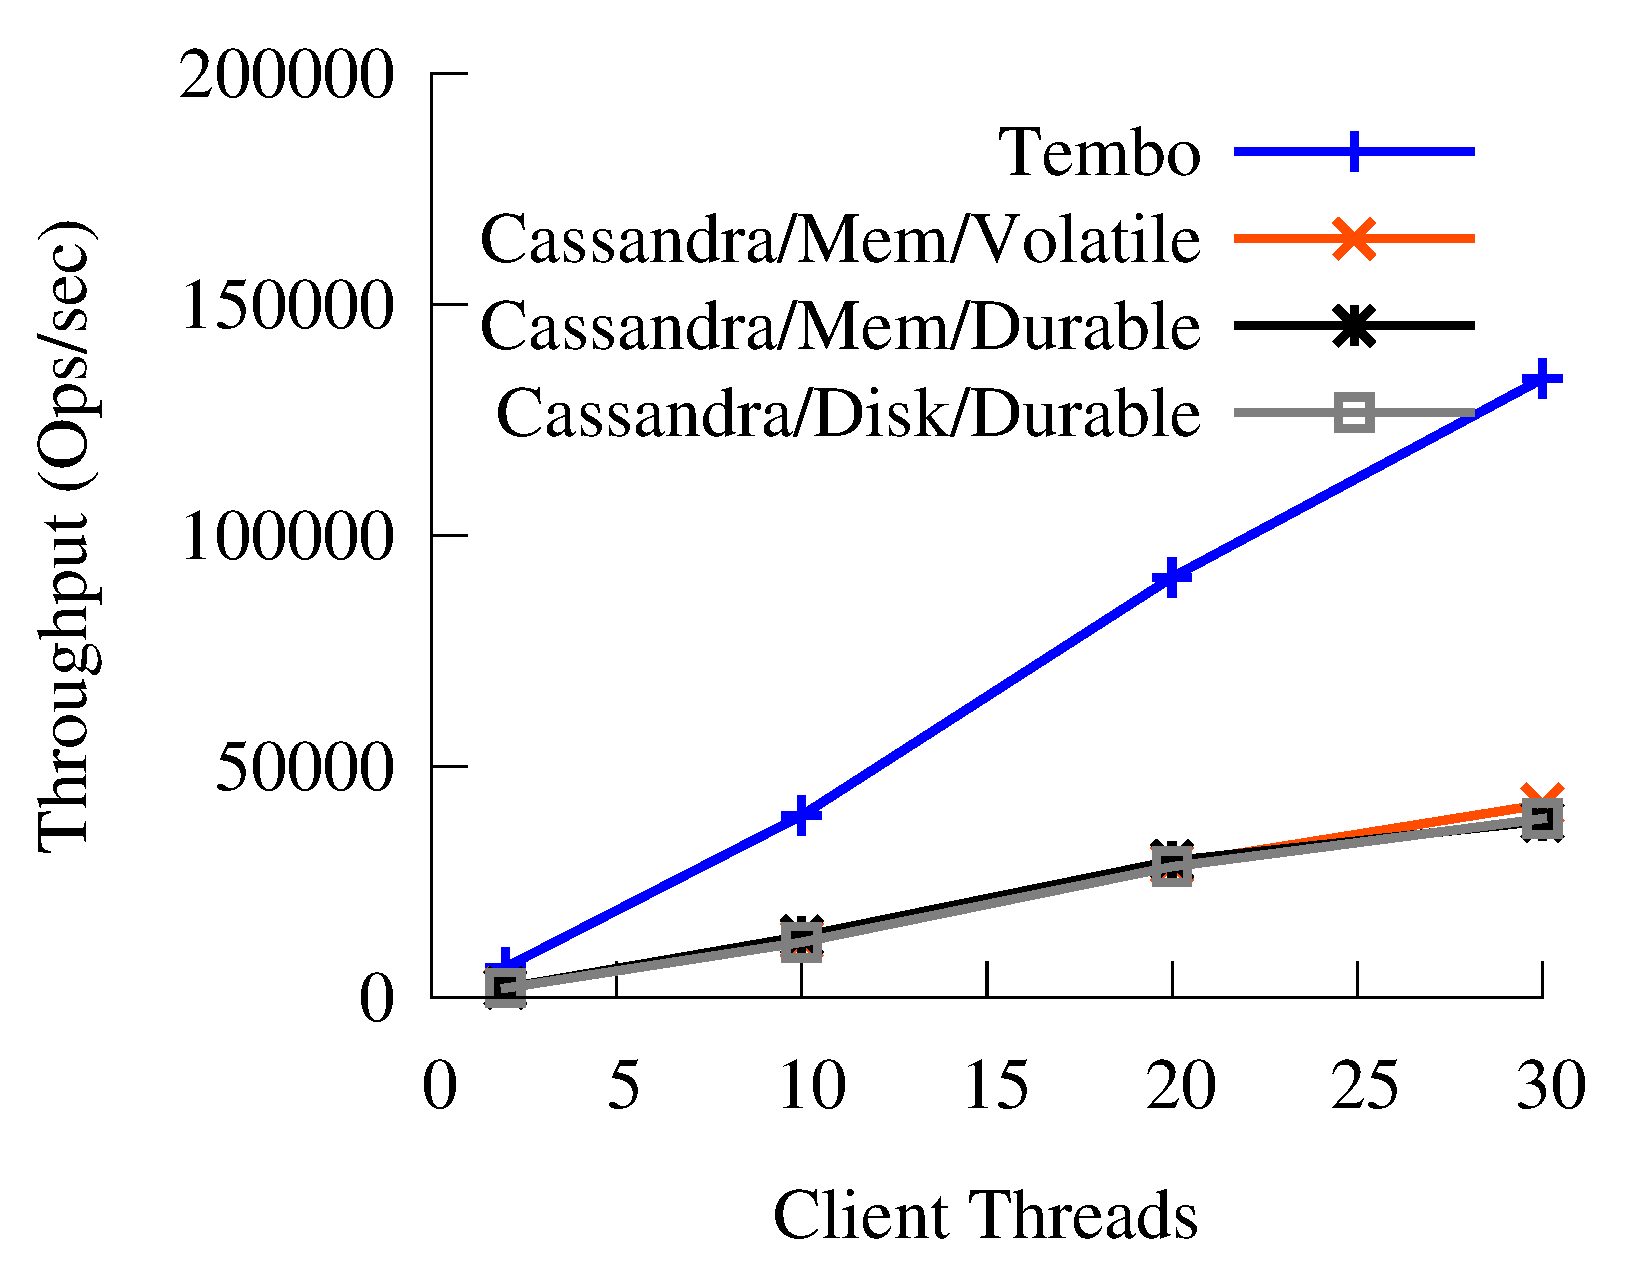
\includegraphics[width=0.85\columnwidth]{figs/ycsb-d}}
\begin{captiontext}
\centerline{Mean of 5 trials. Max.\ standard deviation: 8.1\% of the
  mean.}
\end{captiontext}
\caption[Yahoo Cloud Serving Benchmark: StatusUpdates]{YCSB: StatusUpdates}
\label{fig:ycsb_status_updates}
\end{minipage}
\end{figure}

\section{End-to-End Comparison}


For an end-to-end test, we used YCSB, a framework for evaluating the
performance of Key-Value, NoSQL, and cloud storage systems~\citep{Cooper10}.
In this experiment, we used 13 servers for the cluster and 2 servers
as the clients.  We extended YCSB to support Tembo, and present
results from two of YCSB's workloads.  Workload-A, referred to as
SessionStore in this section, contains a 50:50 read:update mix and is
representative of tracking recent actions in an online user's session.
Workload-D, referred to as StatusUpdates, has a 95:5 read:insert mix.
It represents people updating their online status (e.g., Twitter
tweets or Facebook wall updates) and other users reading them.  Both
workloads execute 2M operations on values consisting of 10 columns
with 100~byte fields.

We compare Tembo to Cassandra (v0.6.1)~\citep{Lakshman10}, a
distributed data store that borrows concepts from
BigTable~\citep{Chang08} and Dynamo~\citep{DeCandia07}.  We used three
different Cassandra configurations in this experiment.  The first two
used a ramdisk for storage but the first (Cassandra/Mem/Durable)
flushed its commit log before every update while the second
(Cassandra/Mem/Volatile) only flushed the log every 10 seconds.  For
completeness, we also configured Cassandra to use a disk as the
backing store (Cassandra/Disk/Durable).

Figure~\ref{fig:ycsb_session_store} presents the aggregate throughput
for the SessionStore benchmark. With 30 client threads, Tembo's
throughput was $286$\% higher than memory-backed durable Cassandra.
Given Tembo and Cassandra's different design and implementation
choices, the experiment shows the overheads of Cassandra's in-memory
``memtables,'' on-disk ``SSTables,'' and a write-ahead log,
vs.\ Tembo's single-level store.  Disk-backed Cassandra's throughput
was only 22--44\% lower than the memory-backed durable configuration.
The large number of disks in our experimental setup and a 512~MB
battery-backed disk controller cache were responsible for this
better-than-expected disk performance.  On a different machine with
fewer disks and a smaller controller cache, disk-backed Cassandra
bottlenecked with 10~client threads. Formal performance 
models~\cite{Varki04} designed for disk arrays have also shown the 
benefits of using battery-backed disk controller caches.

 
Figure~\ref{fig:ycsb_status_updates} shows that, for the StatusUpdates
workload, Tembo's throughput is up to 250\% higher than memory-backed
durable Cassandra.  Tembo's improvement is slightly lower than the
SessionStore benchmark because StatusUpdates insert operations update all
10 columns for each value, while the SessionStore only selects one random
column to update.  Finally, as the entire data set can be cached in
memory and inserts represent only 5\% of this workload, the different
Cassandra configurations have similar performance.


% LocalWords:  Condit NVBM AMD SAS ramdisk mfence Versioning TinySTM GC GHz DL
% LocalWords:  Hans's versioning versioned unversioned Redis YCSB Xeon  Tembo
% LocalWords:  MultCallFlushLRU clflush multi Nehalem versioning's Proliant API
% LocalWords:  NoSQL online BigTable memtables SSTables Tembo's Gigabit CDDS KV
% LocalWords:  cacheline Microbenchmark BDB tuples BDB's ing STX tradeoff HMSET
% LocalWords:  hashtable syscall tradeoffs dels sloccount lookup VTune noop STL
% LocalWords:  Oprofile Microbenchmarks Facebook SessionStore StatusUpdates UNC
% LocalWords:  bottlenecked SNP CDDSs runtime lookups loopback CDDS's YCSB's
% LocalWords:  hashtables tmpfs fsync
